\noindent
\begin{minipage}[t]{0.26\textwidth}
    \begin{tcolorbox}[
        colback=white,
        colframe=stewartgreen,
        arc=0mm,
        boxrule=0.8pt,
        left=5pt,
        right=5pt,
        top=5pt,
        bottom=5pt
    ]
    {\fontsize{9pt}{11pt}\selectfont\textbf{\textsf{\color{stewartgreen}L’Hospital}}\par}
    \vspace{3pt}
    {\fontsize{8pt}{10.5pt}\selectfont\raggedright
    Quy tắc l’Hospital được đặt theo tên của một quý tộc người Pháp, Hầu tước de l’Hospital (1661--1704), nhưng lại được phát hiện bởi nhà toán học người Thụy Sĩ John Bernoulli (1667--1748). Đôi khi bạn có thể thấy tên l’Hospital được viết là l’Hôpital, nhưng chính ông đã tự viết tên mình là l’Hospital, theo thói quen phổ biến vào thế kỷ 17. Xem Bài tập 85 để biết ví dụ mà Hầu tước đã dùng để minh họa quy tắc của mình. Xem dự án tiếp sau mục này để biết thêm các chi tiết lịch sử.\par}
    \end{tcolorbox}

    \vspace{5.5cm}

    \noindent
    \begin{minipage}{\linewidth}
    \fontsize{8pt}{10.8pt}\selectfont\raggedright
    \prohibitionicon\enspace \textbf{Lưu ý rằng} khi sử dụng quy tắc l’Hospital, chúng ta lấy đạo hàm của tử số và mẫu số một cách \textit{riêng biệt}. Chúng ta \textit{không} sử dụng Quy tắc đạo hàm của thương (Quotient Rule).
    \end{minipage}

    \vspace{1.0cm}

    \noindent
    \begin{minipage}{\linewidth}
    \fontsize{8pt}{10.8pt}\selectfont\raggedright
    Đồ thị của hàm số trong Ví dụ 2 được thể hiện trong Hình 2. Trước đây chúng ta đã nhận thấy rằng hàm số mũ tăng nhanh hơn nhiều so với hàm lũy thừa, vì vậy kết quả của Ví dụ 2 không nằm ngoài dự đoán. Xem thêm Bài tập 75.
    \end{minipage}

    \vspace{0.4cm}

    \begin{center}
    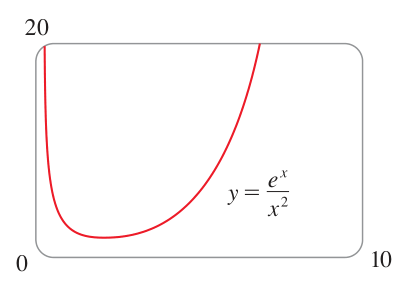
\includegraphics[width=\linewidth]{images/p0346_fig1.png}\\[3pt]
    {\fontsize{8.5pt}{10.5pt}\selectfont\textbf{\textsf{HÌNH 2}}}
    \end{center}
\end{minipage}%
\hfill
\begin{minipage}[t]{0.71\textwidth}
    \noindent\textbf{\textsf{\color{stewartgreen}LƯU Ý 2}}\quad Quy tắc l’Hospital cũng đúng cho các giới hạn một bên và các giới hạn tại vô cực hoặc âm vô cực; nghĩa là, ``$x \to a$'' có thể được thay thế bởi bất kỳ ký hiệu nào trong số $x \to a^+$, $x \to a^-$, $x \to \infty$, hoặc $x \to -\infty$.

    \vspace{0.8em}
    \noindent\textbf{\textsf{\color{stewartgreen}LƯU Ý 3}}\quad Đối với trường hợp đặc biệt khi $f(a) = g(a) = 0$, $f'$ và $g'$ liên tục, đồng thời $g'(a) \neq 0$, ta rất dễ hiểu tại sao quy tắc l’Hospital lại đúng. Thật vậy, sử dụng dạng tương đương của định nghĩa đạo hàm (2.7.5), ta có
    \begin{align*}
    \lim_{x \to a} \frac{f'(x)}{g'(x)} &= \frac{f'(a)}{g'(a)} = \frac{\lim\limits_{x \to a} \dfrac{f(x) - f(a)}{x - a}}{\lim\limits_{x \to a} \dfrac{g(x) - g(a)}{x - a}} \\[7pt]
    &= \lim_{x \to a} \frac{\dfrac{f(x) - f(a)}{x - a}}{\dfrac{g(x) - g(a)}{x - a}} \\[7pt]
    &= \lim_{x \to a} \frac{f(x) - f(a)}{g(x) - g(a)} = \lim_{x \to a} \frac{f(x)}{g(x)} \qquad {\color{stewartcyan}[\text{vì } f(a) = g(a) = 0]}
    \end{align*}

    \vspace{0.2em}
    \noindent Việc chứng minh phiên bản tổng quát của quy tắc l’Hospital phức tạp hơn nhiều. Xem Phụ lục F.

    \vspace{1.1em}
    \noindent\textbf{\textsf{\color{stewartcyan}VÍ DỤ 1}}\quad Tìm $\lim\limits_{x \to 1} \dfrac{\ln x}{x - 1}$.

    \vspace{0.4em}
    \noindent\textbf{\textsf{\color{stewartcyan}LỜI GIẢI}}\quad Vì
    \[
    \lim_{x \to 1} \ln x = \ln 1 = 0 \qquad \text{và} \qquad \lim_{x \to 1} (x - 1) = 0
    \]
    giới hạn này là một dạng vô định kiểu $\frac{0}{0}$, do đó chúng ta có thể áp dụng quy tắc l’Hospital:
    \begin{align*}
    \lim_{x \to 1} \frac{\ln x}{x - 1} &= \lim_{x \to 1} \frac{\dfrac{d}{dx}(\ln x)}{\dfrac{d}{dx}(x - 1)} = \lim_{x \to 1} \frac{1/x}{1} \\[7pt]
    &= \lim_{x \to 1} \frac{1}{x} = 1 \tag*{\color{stewartcyan}\blacksquare}
    \end{align*}

    \vspace{0.7em}
    \noindent\textbf{\textsf{\color{stewartcyan}VÍ DỤ 2}}\quad Tính $\lim\limits_{x \to \infty} \dfrac{e^x}{x^2}$.

    \vspace{0.4em}
    \noindent\textbf{\textsf{\color{stewartcyan}LỜI GIẢI}}\quad Ta có $\lim\limits_{x \to \infty} e^x = \infty$ và $\lim\limits_{x \to \infty} x^2 = \infty$, do đó giới hạn có dạng vô định kiểu $\frac{\infty}{\infty}$, và quy tắc l’Hospital cho ta
    \[
    \lim_{x \to \infty} \frac{e^x}{x^2} = \lim_{x \to \infty} \frac{\dfrac{d}{dx}(e^x)}{\dfrac{d}{dx}(x^2)} = \lim_{x \to \infty} \frac{e^x}{2x}
    \]
    Vì $e^x \to \infty$ và $2x \to \infty$ khi $x \to \infty$, nên giới hạn ở vế phải cũng là một dạng vô định. Áp dụng quy tắc l’Hospital lần thứ hai, ta được
    \[
    \lim_{x \to \infty} \frac{e^x}{x^2} = \lim_{x \to \infty} \frac{e^x}{2x} = \lim_{x \to \infty} \frac{e^x}{2} = \infty \tag*{\color{stewartcyan}\blacksquare}
    \]
\end{minipage}
